%%%%%%%%%%%%%%%%%%%%%%%%%%%%%%%%%%%%%%%%%
% Paper Notes
% LaTeX Template
% Version 1.0 (25/10/18)
%
% Author: Fred Guth (fredguth@fredguth.com
%
% License:
% CC BY-NC-SA 3.0 (http://creativecommons.org/licenses/by-nc-sa/3.0/)
%
%%%%%%%%%%%%%%%%%%%%%%%%%%%%%%%%%%%%%%%%%

%----------------------------------------------------------------------------------------
%	PACKAGES AND OTHER DOCUMENT CONFIGURATIONS
%----------------------------------------------------------------------------------------

\documentclass[
10pt, % Default font size is 10pt, can alternatively be 11pt or 12pt
a4paper, % Alternatively letterpaper for US letter
onecolumn, % Alternatively twocolumn
% portrait % Alternatively landscape
]{article}

%%%%%%%%%%%%%%%%%%%%%%%%%%%%%%%%%%%%%%%%%
% Paper Notes
% Structure Specification File
% Version 1.0 (25/10/18)
%
% Author: Fred Guth (fredguth@fredguth.com
%
% License:
% CC BY-NC-SA 3.0 (http://creativecommons.org/licenses/by-nc-sa/3.0/)
%
%%%%%%%%%%%%%%%%%%%%%%%%%%%%%%%%%%%%%%%%%%%%%%%%%%%%%%%%%%%%%%%%%%%%%%%%%%%%%%%%%%

%----------------------------------------------------------------------------------------
%	REQUIRED PACKAGES
%----------------------------------------------------------------------------------------

\usepackage[includeheadfoot,columnsep=2cm, left=1in, right=1in, top=.5in, bottom=.5in]{geometry} % Margins

\usepackage[utf8]{inputenc}
\usepackage{XCharter} % XCharter as the main font
\usepackage{booktabs}
\usepackage{natbib} % Use natbib to manage the reference
\usepackage{bibentry}
\usepackage{graphicx}
\graphicspath{{./assets}{assets/}}%
\nobibliography*
\bibliographystyle{plain} % Citation style

\usepackage[english]{babel} % Use english by default

%----------------------------------------------------------------------------------------
%	CUSTOM COMMANDS
%----------------------------------------------------------------------------------------
\newcommand{\horrule}[1]{\rule{\linewidth}{#1}} % Create horizontal rule command with 1 argument of height
\newcommand{\papertitle}[1]{\renewcommand{\papertitle}{#1}} % Define a command for storing the article title
\newcommand{\papercitation}[1]{\renewcommand{\papercitation}{#1}} % Define a command for storing the article citation
% \newcommand{\doctitle}{``\papertitle''\---\papercitation  } % Define a command to store the article information as it will appear in the title and header

\newcommand{\datenotesstarted}[1]{\renewcommand{\datenotesstarted}{#1}} % Define a command to store the date when notes were first made
\newcommand{\docdate}[1]{\renewcommand{\docdate}{#1}} % Define a command to store the date line in the title

\newcommand{\docauthor}[1]{\renewcommand{\docauthor}{#1}} % Define a command for storing the article notes author

% Define a command for the structure of the document title
\newcommand{\printtitle}{

\begin{center}

  \horrule{0.5pt} \\[0.4cm] % Thin top horizontal rule

  \bigskip

  \textbf{\Large{"\papertitle"}}

  \papercitation 

  \bigskip
  
  \docdate

  \docauthor

  \bigskip
  

  \horrule{2pt} \\[0.5cm] % Thick bottom horizontal rule

\end{center}


}

%----------------------------------------------------------------------------------------
%	STRUCTURE MODIFICATIONS
%----------------------------------------------------------------------------------------

\setlength{\parskip}{3pt} % Slightly increase spacing between paragraphs

% Uncomment to center section titles
%\usepackage{sectsty}
%\sectionfont{\centering}

% Uncomment for Roman numerals for section numbers
%\renewcommand\thesection{\Roman{section}}
 % Input the file specifying the document layout and structure

%----------------------------------------------------------------------------------------
%	ARTICLE INFORMATION
%----------------------------------------------------------------------------------------

\papertitle{Unbiased Look at Dataset Bias} % The title of the article you are reviewing
               
\papercitation{\bibentry{Torralba2011}} % The BibTeX reference of the article you are reviewing

\datenotesstarted{October 29, 2018} % The date when these notes were first made
\docdate{\datenotesstarted; rev. \today} % The date when the notes were lasted updated (automatically the current date)

\docauthor{Fred Guth} % Your name

%----------------------------------------------------------------------------------------
% No need to change this part
\begin{document}
\pagestyle{myheadings}
\markright{\papertitle} % Place the article information into the header

%----------------------------------------------------------------------------------------
%	PRINT ARTICLE INFORMATION
%----------------------------------------------------------------------------------------
% No need to change this part
\thispagestyle{plain} % Plain formatting on the first page

\printtitle % Print the title

%----------------------------------------------------------------------------------------
%	ARTICLE NOTES
%----------------------------------------------------------------------------------------
% Here is where you edit
\section*{Summary} 

\begin{description}
\item[Purpose] The access to large image datasets has been a key driver on the recent progress on Computer Vision tasks like object detection or face recognition. Despite its important role and the authors best efforts, all datasets evaluated by the paper presented strong built-in bias and, in a way, failed in the objective of representing the real world. 

The basic question that drives this paper is: \textit{Are the datasets measuring the expected performance in the real world?} Computer vision datasets have become closed worlds unto themselves and achieving a good benchmark in one, just means you are overfitting your model to that domain. 

The goals of this paper are:
\begin{enumerate}
    \item show how bias sneaks into datasets and affects tasks performance;
    \item raise awareness to this important issue that had been neglected.
\end{enumerate}


\item[Claims] The authors claim that: 
\begin{itemize}
\item due to built-in biases datasets are failing in the general goal of representing the real world;
\item some datasets like Caltech and MSRC are not helpful anymore and should be avoided;
\item even automatically collected internet images present bias, as most results of searches bring photos where the searched term is occupying the center/focus of the picture. 
\item rich and unbiased negative set is important to classifier performance;

\end{itemize}
\item[Experiments and Conclusions] The authors used the SOTA object detection of that time, 2011 (no convolutional network).  To minimize \textit{selection bias}, they picked 2 objects common to all datasets, "car" and "person". Each classifier was trained with 500 positive and 2000 negative for the classification task and 100 positive and 1000 negative for the detection task for each dataset. Test was performed with 50 positive and 1000 negative examples for classification and 10 positive and 20000 negative for detection. For testing, each classifier was run 20 times and results were averaged.
\begin{figure}[!htp]
    \centering
    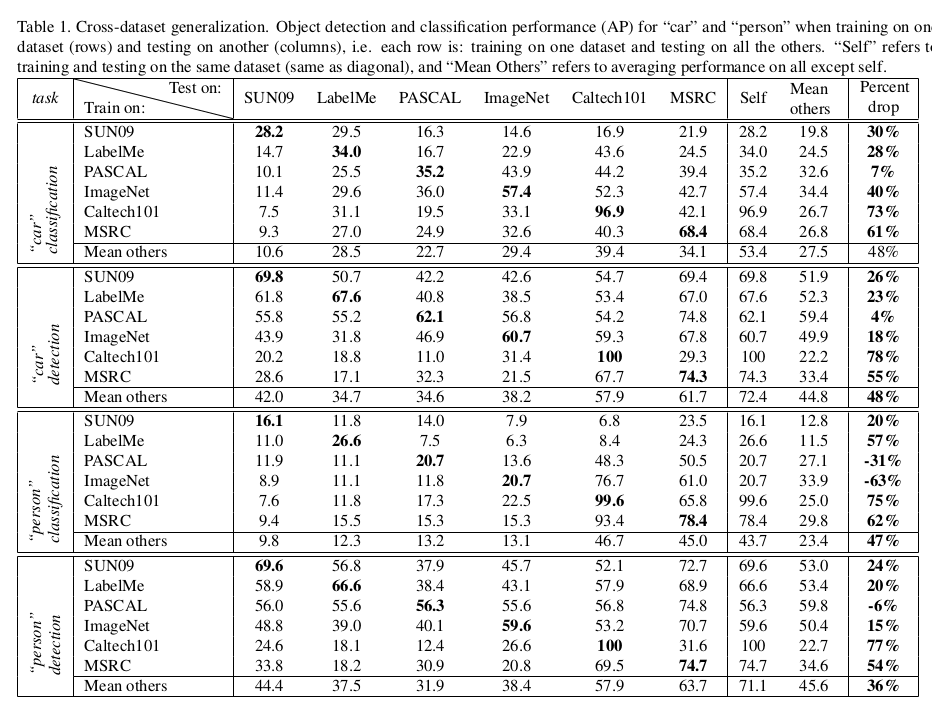
\includegraphics[width=.8\textwidth]{table1}
    \label{table1}
\end{figure}
The results were depressing, little generalization cross datasets as shown in the table \ref{table1}.

To evaluate relative bias in negative sets of the datasets, they created a superset of negatives of all datasets and, for each dataset, trained the classifier with positive and negative samples from its own dataset and tested with positives of the dataset and negatives from the superset. The number of samples obeyed the previous experiment protocol. There was a significant loss in performance, where negatives from other datasets were classified as positives. ImageNet, Caltech and MSRC did not show a drop in results for different reasons.  ImageNet seems to have a large variability of negatives, the others just seem to be too easy.
\end{description}

%------------------------------------------------

\section*{Evaluation}

The authors raised awareness for an important problem. With so much hype on the "success" of Deep Learning to all sorts of Computer Vision tasks, it is easy to forget that even good and large datasets like ImageNet present bias and fail to represent the real world.  Consequently, deep learning research and practitioners, includind us, treat every new real world application data as a new domain that needs to be fine-tunned, alas our best datasets are far to be good enough for general usage. Although being impossible to build a dataset without bias, the problems pointed were pertinent. 

They showed that even in the presence of strong bias, Caltech and MSRC were easy to be classified, therefore they do not provide much value nowadays (2011).

They have clearly experimentaly proved their claims and a quick search on Google Scholar shows that they achieved their goal of raising awareness to the problem: not only the paper has more than 770 citations, but since its publication, several other papers on the subject of dataset bias were published. 


%------------------------------------------------

\section*{Synthesis}


For my research, I believe the paper helped me realize that we humans also have access to biased input, but are able to much more efficiently generalize our learnings. This is an indication that even in areas where it seems that our SOTA have great results, we are quite far from what is possible. 

The use of unbalanced positive and negative datasets by an order of magnitude made me wonder my own dataset building choices and negative set bias. 

Another important point is that the area has seen major improvements due to better datasets and dataset engineering should be better researched. 

%
%----------------------------------------------------------------------------------------
%
%----------------------------------------------------------------------------------------
%	BIBLIOGRAPHY
%----------------------------------------------------------------------------------------

\renewcommand{\refname}{References} % Change the default bibliography title

\bibliography{references} % Input your bibliography file

%----------------------------------------------------------------------------------------

\end{document}